\documentclass[11pt]{article}
\usepackage[margin=1in]{geometry}
\usepackage{graphicx}

\linespread{1.4}

\begin{document}
\begin{center}
{\Large \textbf{Collaborative Research: Resource of Open\\
Problems for Education (ROPE)}}
\end{center}

\begin{section}{Introduction}

At the heart of teaching and learning mathematics---and many other
disciplines---is a learner's engagement with questions, or problems, which
challenge her/him to understand and apply the material s/he is
learning.  We propose to develop a resource that will provide an online
electronic library of innovative, well-tested, and documented problems
that instructors and students may use in a wide range of courses and for a
wide range of assignment types.  This ``Resource of Open Problems for
Education'' (ROPE) will allow searching and browsing to find useful
problems; will use information about problem usage and user endorsements
to provide a collaborative, ``crowd-sourced,'' vetting process for problems;
and will allow users to share collections of problems drawn from the
library and groups of such collections.  Because it will be an open
resource, all institutions and individuals regardless of means will have
full access to it, and the community of ROPE users will be able to provide
added value to the resource.  The goals of ROPE are:
\begin{itemize}
  \item
    To be a \textit{free, open-source resource} that will give instructors
    and students access to an extensive collection of good mathematics
    problems.  The cost of textbooks and supporting materials for courses
    is increasingly untenable, and ROPE will be not only an expansive
    resource, but one that does not discriminate on the basis of wealth,
    and which does not demand advertising or private data for its use.
  \item
    To have within this resource a mechanism for users to create
    \textit{collections of problems, and collections of collections,} that
    they may use themselves or share with other users.  This will allow
    instructors to create problem sets, quizzes, and collections of these
    for a course, will allow students to create practice
    worksheets or other study aides, and, at the other end of the
    instructional spectrum, will allow authors to define groups of
    problems that complement their text.
  \item
    To develop a \textit{community of users} of these problems, who may
    contribute problems and related content, may provide feedback on
    problems, and may share with other users the collections they have
    created.
\end{itemize}
With this proposal we seek to develop this core functionality and a
sustainable user community for ROPE, which will provide the base from
which we may refine and further extend the system.

\end{section}

\begin{section}{Description}

Internet users go to Amazon to search for products to buy, and to
Google to find information on the Web.  While we do not pretend to be
creating a resource with the ubiquity or power of either of those, we do
hope to develop ROPE into the place where mathematics teachers and
learners go to find problems and inspiration for problems for the courses
they are teaching and learning, respectively.  We imagine going to the
ROPE search page, such as is suggested in Figure~\ref{rope1}, and
searching for a topic or problem, with the result suggested in
Figure~\ref{rope2}.  These mock-ups illustrate a number of the core
features that ROPE will have:

\begin{figure}
\begin{center}
\framebox{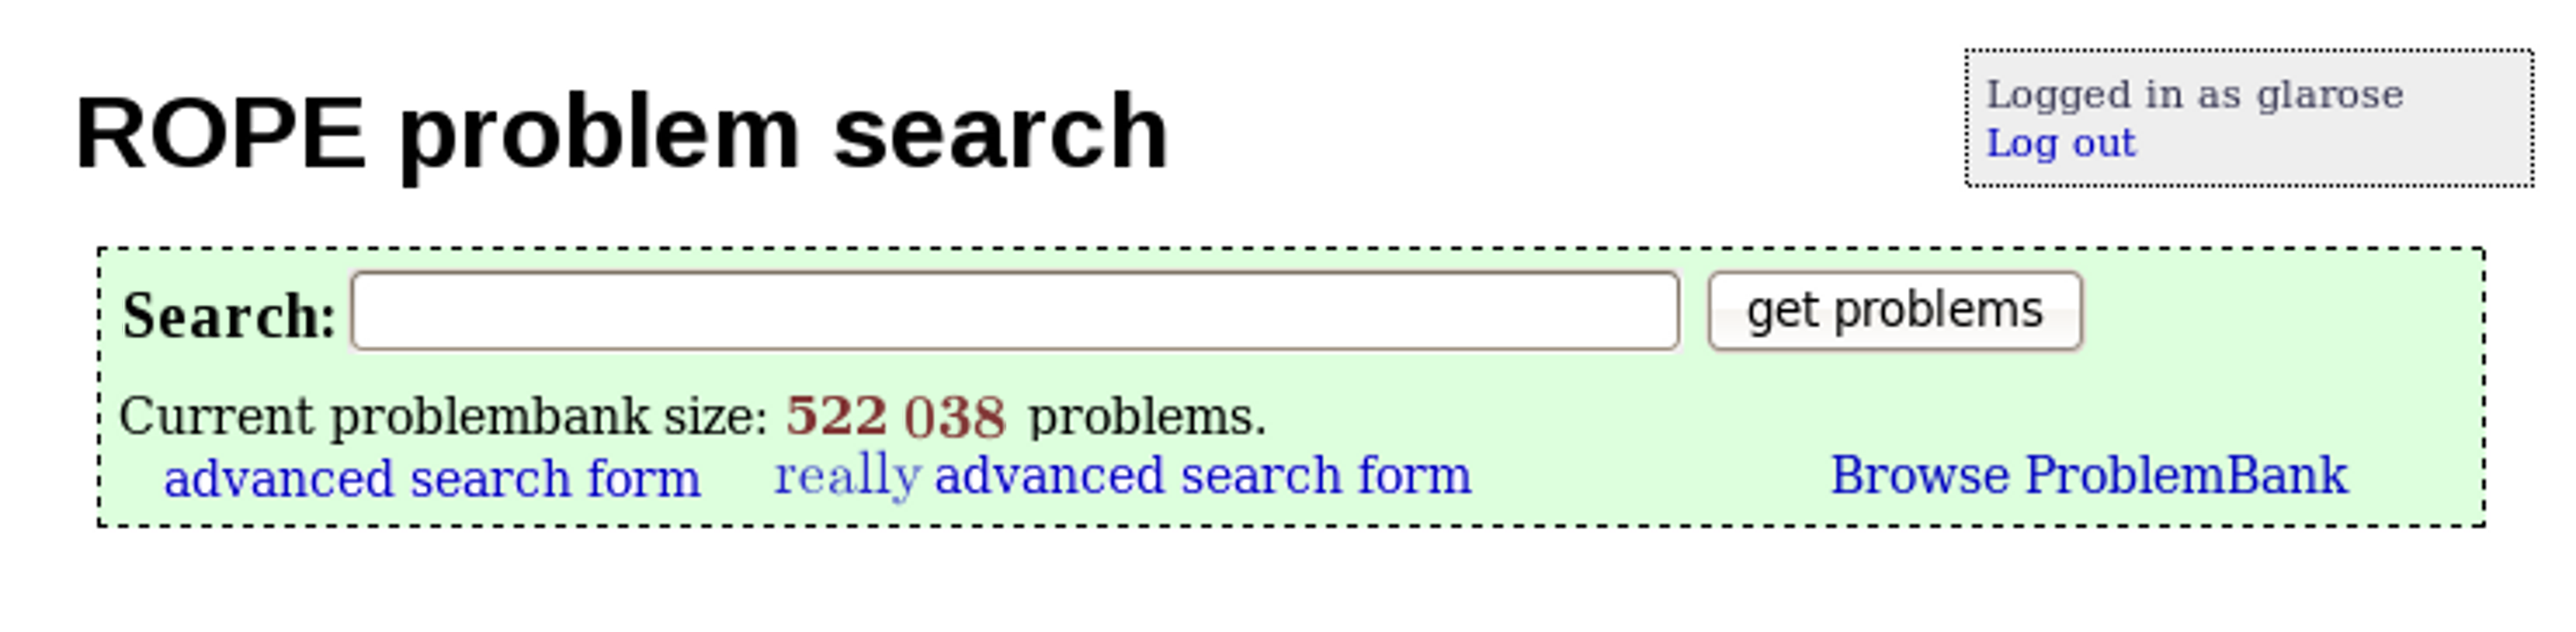
\includegraphics[width=4.25in]{rope_search}}\\
\caption{Mock-up of ROPE search page}
\label{rope1}
\end{center}
\end{figure}

\begin{figure}
\begin{center}
\framebox{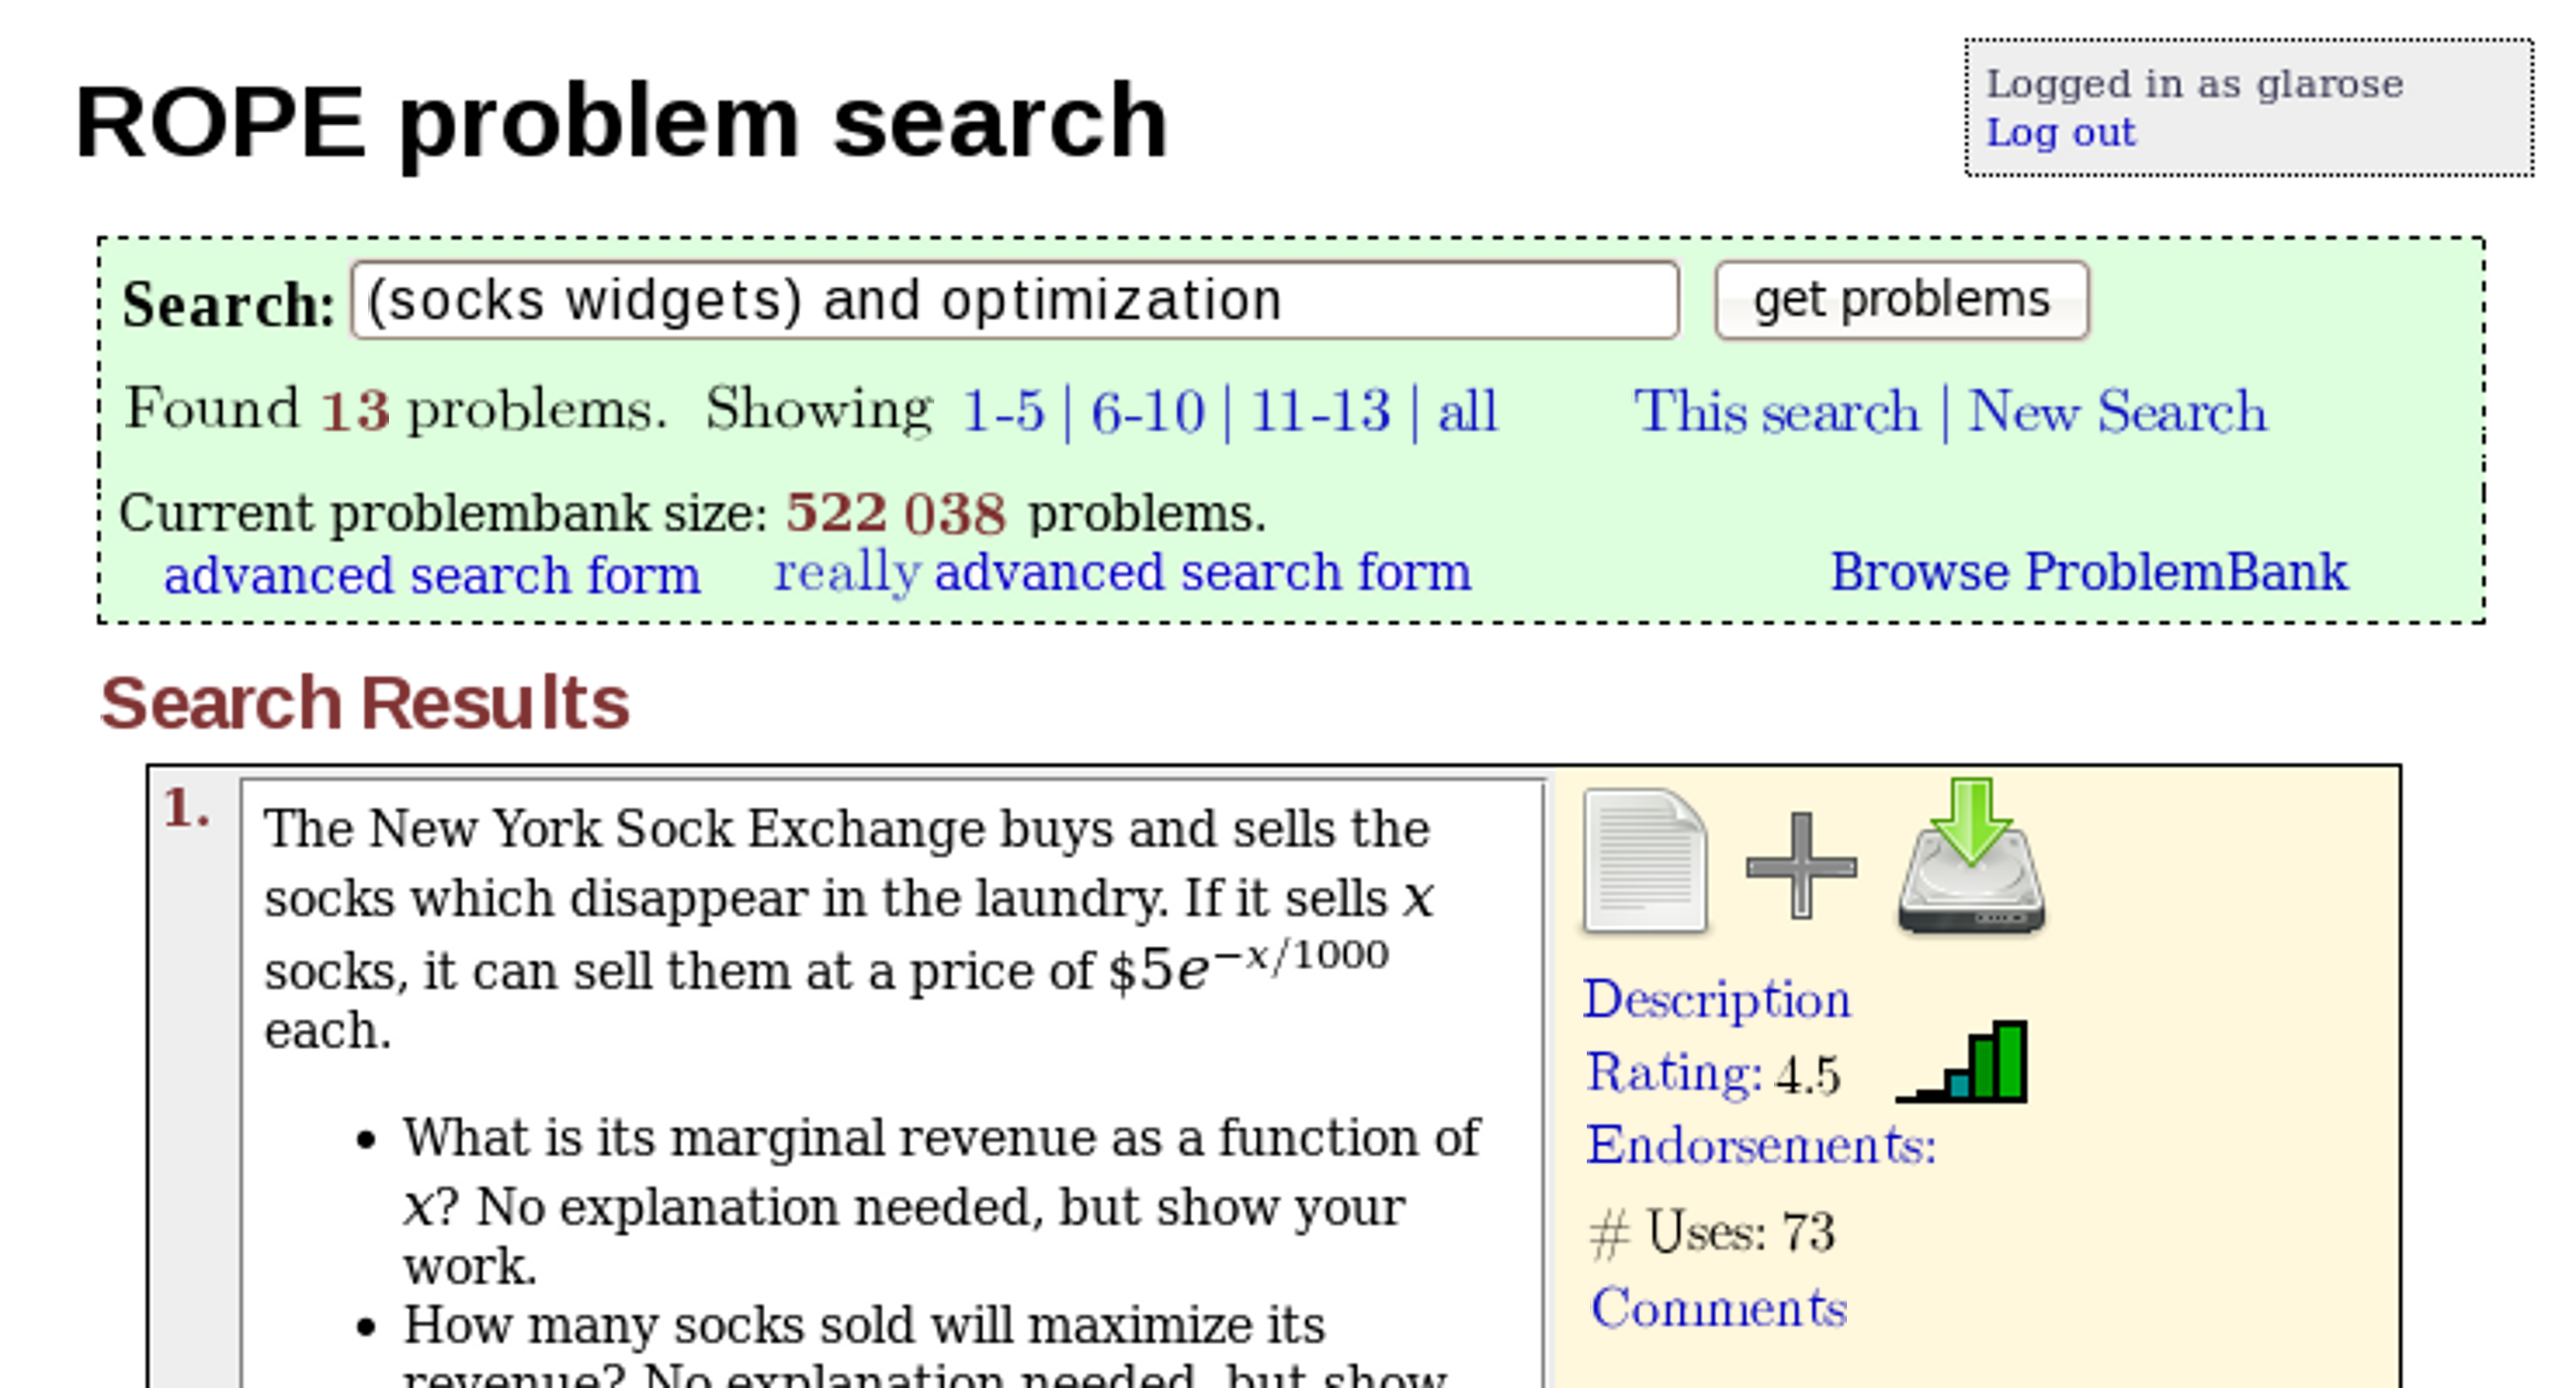
\includegraphics[width=4.25in]{rope_search_results}}\\
\caption{Mock-up of ROPE results page}
\label{rope2}
\end{center}
\end{figure}

\begin{list}{$\bullet$}{\setlength{\parsep}{0pt}\setlength{\itemsep}{0pt}}
  \item
    Users will be able to search on arbitrary keywords, or with Gmail or
    Google-like tags (e.g., ``course:calculus''), and there will be
    alternate search forms that will allow users to explicitly select
    specific courses, chapter or section headings, etc.  This search will
    be available to anyone, without requiring that they log in to the site
    or provide any information.  The other user features described below
    will necessarily require that users establish a username and account
    in ROPE so that data may be stored for them, but the data collected
    will be little more than a username and e-mail address.
  \item
    Search results will be easily managed, with a view of the problems and
    easy ways to view the source (e.g., \LaTeX) for the problems, add them
    to Problem Collections owned by the user, and download them as a small
    file.
  \item
    All problems will have useful metadata that describe them, including
    the background mathematics required for the problem (e.g., calculus
    and optimization), level of difficulty (e.g., easy, medium, hard),
    type of problem (e.g., symbolic, numerical, graphical), etc.
  \item
    Users will be able to rate problems, endorse them, and leave comments,
    and these data and other usage data will be used to help organize
    search results and will be available also to allow other users to
    evaluate the problems and how they might be used. 
  \item
    Users will have the ability to build their own problem collections and
    share them with other users, and to download a full source file (e.g.,
    in \LaTeX) for a problem set, other assignment, or even the full list
    of all problem sets they have created for a course. 
\end{list}

In the following we illustrate these core features with three ``use
cases'': how instructors, students and authors might use the resource.

%% In the following we discuss the three key functionalities we envision for
%% ROPE: the searchable problem library, from which users may view and
%% download problems; the ability to create collections and collections of
%% collections; and its community of users and how that will integrate with
%% the other two features.  In a final section we discuss some of the
%% extensions and technical details that we expect to make ROPE as flexible,
%% useful, and usable as possible.

%% old sections moved below the \end{document}

\begin{subsection}{Authors' Use}

An author is writing an open Linear Algebra text, and decides to use ROPE
as a source for the problems she includes at the end of each section of
her text.  She creates a collection in ROPE for her text, and within that
collections for each chapter and section.  Using ROPE's search tool, she
finds problems that she likes for each section of her book and uses the
information about the problems to group those in order of difficulty and
by type of problem.  In selecting the problems she uses both this metadata
and the information about other ROPE users' ratings, comments, and the
number of uses that the problems have seen.  For some sections of her
text she finds that the problems available in ROPE do not include all
aspects of the material she wants to have covered, and so adds to ROPE
some problems to complete the problem sets for those sections.  She then
makes the problem collections she has created for the text public, and
puts links to them and to the problems in them in her text.

\end{subsection}

\begin{subsection}{Instructors' Use}

An instructor is using a popular calculus textbook from a well-established
publisher.  His university uses a web homework system that includes
problems from that text, so he assigns web homework from that system.  In
addition, however, he wants to have some written assignments, and to
augment the problems available in the textbook he uses ROPE to find
related problems that fill in gaps he sees in the textbook's coverage of
some of the topics.  He creates a personal problem collection in ROPE with
all of these problems so that he can easily find them again, and includes
them in his assignments by copying the \LaTeX\ code for the problems from
ROPE into his \LaTeX ed homeworks.  Each week he gives a quiz to his
class, and searches ROPE for problems to modify for his quizzes.  For
quizzes he copies the \LaTeX\ for the problems and then changes it to give
problems that he thinks are at the appropriate level for his students.
When searching for problems he is able to use other users' comments and
ratings to anticipate where his students may have trouble, and for those
problems he finds to be particularly effective he adds some comments and
positive ratings.  When the semester ends, he shares his problem
collection with the instructor who is teaching the course in the following
semester so that she can see which problems he used.

\end{subsection}

\begin{subsection}{Students' Use}

A student is taking the differential equations course at her college, for
which her instructor has the usual collection of on-line and written
homework, quizzes and exams.  Before the exams, the student uses ROPE to
assemble some study guides consisting of problems covering the material
for which she will be responsible.  She uses ROPE's search tool to find
problems that cover the right material, and makes a problem collection in
ROPE for each study guide.  Because these are natively \LaTeX\ documents,
she is able easily to download a PDF of each study guide from which to
study.  As a separate document she creates a version of the study guides
that include the answers and solutions to the problems she selected, where
they are available.  Later she shares her study guide problem collections
with friends in the course so that they are able to use them when studying
for the final.

\end{subsection}

\begin{subsection}{Use Case Observations}

As can be seen from these use cases, the power and usefulness of ROPE is
rooted in its ability to provide a broad, searchable, library of problems
with descriptive data and information about use and usefulness of the
problems, and the manner in which it allows users to create collections of
these problems for their and others' use and future use.  The fact that it
is an open resource is a key to this: there is no restriction on who can
use these problems, and there is no subscription fee or hurdle preventing
its use.  It may be noted that as a result of this openness the instructor
using problems from ROPE might worry about his students finding the
problems or solutions as well.  In the face of the ready availability of
resources such as Wolfram$|$Alpha, Yahoo Answers and---even
worse---StackOverflow, however, we feel this concern is largely beside the
point.  In today's world a student can find the solution to any problem we
assign (from calculus to graduate topology proofs) on-line, and the
availability of ROPE will not affect that.  ROPE will provide a resource
that can be used to promote and enhance student learning by making
accessible a searchable library containing many well-described, effective
problems.

\end{subsection}

\end{section}

\begin{section}{Context}

While there is no resource currently available that provides the
functionality and material that will be included in ROPE, there is
existing software that will provide a basis for it, and which will inform
its development.  Three applications that are closely related to the work
we seek to do with ROPE are: an existing problem library developed in the
mathematics department at the University of Michigan by Gavin LaRose; the
Open Problem Library (OPL) used by the WeBWorK [3] %\cite{webwork}
online
testing and assessment system, for which Gavin LaRose has been a software
developer; and Edfinity [6], a commercial website providing content and
self-publishing options for educators.

The problem library in use at the University of Michigan currently
provides a subset of the features we envision for ROPE: it has an
online, searchable interface that allows users at the University to
search through over 500 problems drawn from precalculus and calculus
homework assignments, quizzes and exams.  Problems are described by
course, chapter, section, keywords, difficulty, type, original use, year
used, author, and general math topic.  The experience developing the
underlying data structures and interface for this will be of great use in
the development of ROPE, and we expect to be able to reuse some
portions of its programming code as ROPE is created.  

The WeBWorK OPL (Open Problem Library) provides a similar search
functionality for over 22,000 problems written for WeBWorK, and is
integrated into WeBWorK to allow creation of problem sets from those
problems through a library browser interface.  But it is, necessarily,
strictly a resource of problems for WeBWorK, and therefore does not
provide the flexibility and extensibility that we envision for ROPE.  It
is worth mentioning that the types of problems that we envision for ROPE
extend beyond those that are appropriate for WeBWorK.  Nonetheless, we do
expect that the data structures used in and the experience of the creators
of the OPL will provide added insight on the development of ROPE, and its
interface with the WeBWorK system will be of particular use as we consider
the API for ROPE and how that may allow connections with other systems.

Edfinity is similar in some ways to ROPE (and the WeBWorK OPL), in
providing a searchable database of problems with the capability of 
collecting problems into a problem set---and, in the long-term, an on-line
homework delivery system based on WeBWorK.  They also allow authors to 
self-publish problems, with the promise of royalties if the problem is
used frequently by other educators.  However, it is not an open-source
application and does not support the same flexibility in problem
collection creation that we envision for ROPE.

In addition to the Michigan problem bank, WeBWorK's OPL, and Edfinity, there are
other problem collections that have been developed to serve specific
purposes, and we hope to work with the developers and maintainers of those
to enhance ROPE and to build connections with them.  These include the
MathQuest/MathVote question library at Carroll College [1], % \cite{mathquest},
which includes many questions for use with in-class voting systems; the
GoodQuestions project [5], %\cite{goodquestions},
which provides similar types of
questions; and Quadbase [4], %\cite{quadbase},
which is closest in spirit to ROPE but provides more limited options for 
searching and problem format,
and does not support external use or problem sharing, nor the
community feedback aspects that we envision for ROPE.  
% In addition, the
% Mathematical Association of America (MAA), which is the largest
% professional organization supporting the teaching and learning of
% undergraduate mathematics, has been exploring the possibility of creating
% a problem bank for problems found in its journals.  The MAA is also the
% hosting institution for the WeBWorK project.  We have been in discussion
% with the leadership of the MAA about ROPE and will pursue the
% possibility that it can be connected to the idea of a journal problem
% library as well.

In addition to these specific applications that support some subset of
the features of ROPE, there are a growing number of social networking
and shopping sites that provide us with interface design principles that
will be commonly understood and useful to the users of ROPE.  Sites
including Facebook, LinkedIn, and Amazon allow users to ``like'' ideas or
objects, providing a powerful and simple feedback mechanism that informs
others of the popularity and usefulness of the ``liked'' item.  These
sites also allow users to set up collections of objects (like wish lists
and shopping carts) that may be used personally or shared with others.
Our development of the interface for ROPE will be informed by these
sites, and ROPE will adopt these ideas to give users feedback on
problems in the library, and to develop problem collections that they may
use semester to semester and which they may share with colleagues or with
all users of the system.

Finally, we believe that the educational world in which we are working has
reached a tipping point that argues strongly for the development of an open
resource such as ROPE.  There is increasing outcry about the constraints
and disadvantages of commercial products and the cost of higher
education---which is only compounded by the cost of textbooks and other
class resources.  The open-source movement continues to demonstrate that
it is possible for very good content and programs to be
developed collaboratively and openly, and online communities have
increased in significance and impact. 
As more
open-content textbooks become available, ROPE will be able to provide a
problem resource that complements their problems and work.  Programs such
as WeBWorK and projects such as Wikipedia demonstrate that free, open
development can create products and content that are broadly useful, and
which complement and compete effectively with commercial products.  And
communities such as Project NExT [2] and those connecting instructors
using inquiry-based learning have developed into online networks of
college faculty who are actively engaged with the use of available
resources and technology to improve their teaching (e.g., at the Legacy of
R.L.~Moore Conferences [7] and through AIBL [8]).

\end{section}

\begin{section}{Project Implementation and Timeline}

Our timeline to implement ROPE is shown in Figure~\ref{timeline}.  In
summary, we will have an alpha version of the system running after Summer
and Fall 2015, to be tested in Spring 2016.  In Summer 2016 we will
resolve issues that are determined in the alpha test.  During the
2016--2017 academic year the system will be in beta-testing.  Following
Summer 2017 we expect to move the core the system into production.

Each year the PIs will meet twice in person at national meetings.  This
will allow productive discussions to develop the planning and
direction of the project, as well as talks and posters to be presented to
initiate its dissemination.  In each of the first two years the PIs will
meet with the 
Advisory Group, and with the external evaluator (the latter being paired
with the summer meeting).  These visits are front-loaded to maximize the
formative impact of the discussions we have with them.  We
will be meeting online with our external evaluator during the course of the
project and in person once a year.

\begin{figure}
\begin{center}
\begin{tabular}{|l|l|l|l|}
  \hline
  \textbf{Date} & \textbf{Personnel} & \textbf{Activity} & \textbf{Outcome}\\
  \hline
  \hline
  Summer 15 & PIs, AG & On-site meeting (UM) & Develop design
        principles, data outline \\
	    & PIs, Pr & Development & Programming, database development \\
	    & PIs & Meeting (Mathfest) & Assess initial design,
        revise plan \\
            & PIs, EE & On-line meeting & Frame evaluation, required data \\
  \hline
  Fall 15 & PIs, Pr & Development & Programming for alpha backend, UI \\
	  & PIs & User recruitment & Alpha tester recruitment \\
  \hline
  Jan 16 & PIs, EE & Meeting (JMM) & Frame evaluation, data collection\\
  \hline
  Spring 16 & PIs, AG, EE & On-line meeting & Initial program assessment \\
            & PIs, At & Alpha testing & Alpha testing of resource \\ 
	    & PIs, At & Library development & Expansion of library \\
            & PIs, Pr & Programming work & Debugging alpha code \\
  \hline 
  Sum 16 & PIs, AG, EE & On-site meeting (NAU) & Evaluation, develop
    moderation model \\ 
	    & PIs, Pr & Development & Develop beta software \\
	    & PIs, AG & On-line meeting & Evaluate beta software \\
	    & PIs & User recruitment & Beta tester recruitment \\
	    & PIs & Meeting (Mathfest) & Planning, publicity \\
  \hline
  Fall 16 % & PIs & On-line meeting  & Assessment, obstacle
	  % identification\\
	    & PIs, Bt & Beta testing & Beta testing of resource \\
  \hline
  Jan 17 & PIs, EE & Meeting (JMM) & Evaluation meeting \\
	    & PIs & User Recruitment & Recruit further users \\
  \hline
  Spr 17 & PIs, Bt & Beta testing & Further beta testing of resource \\
	    & PIs, EE & Evaluation & Contact users, solicit feedback \\
  \hline
  Sum 17 & PIs & Development & Debugging and interface revision \\
	    & PIs & Editorial work & Problem moderation,
	documentation \\
	    & PIs, EE & Meeting (Mathfest) & Evaluation and planning,
        dissemination \\
	    & PIs & User recruitment & Recruit additional users\\
  \hline
  Fall 17 & PI & Development & Development, expansion of library \\
  \hline
  Jan 18 & PIs & Meeting (JMM) & Evaluation of moderation, evaluation
	\\ & & & and dissemination; future planning \\
  \hline
  Spr/Sum 18 & PIs & Editorial work & Problem moderation,
	documentation \\ 
  \hline
\end{tabular}
\caption{Project Timeline: personnel notation---PIs = grant PIs; AG =
  Advisory Group; Pr = contract programmer; EE = External Evaluator; At =
  Alpha testers; Bt = Beta testers} 
\label{timeline}
\end{center}
\end{figure}

All programming and software development will be managed by a hired
programming consultant and Gavin LaRose.  Problem creation and expansion
of the problem database will be managed by Dana Ernst and Spencer
Hamblen.  They will also recruit alpha and beta testers, who will be paid
a small honorarium to contribute problems and provide regular feedback on
their use of the system and how it may be improved or how it is working
well.

By the end of its beta development stage, we expect that ROPE will have
a useful number of problems and the core functionality we require of the
system.  Essential functions (problem search,
collections, and the community of users) will be in place for alpha
testing.

Finally, the Math Department at the University of Michigan will be able to
provide the required technical support to initially implement and
subsequently maintain the computer hardware required for this project.
While it is in development and alpha and beta testing, ROPE will be
hosted on web servers that are currently maintained in the Department and
which have the required capacity to support the project.  We discuss
ongoing maintenance and sustainability of ROPE as a production service
below. 

\end{section}

\begin{section}{Project Personnel}

The PIs for 
the grant are Gavin LaRose, University of Michigan, Dana
Ernst, Northern Arizona University and Spencer Hamblen, McDaniel College.

\textbf{Gavin LaRose} is a lecturer~IV and manager of instructional
technology in the Department of Mathematics at the University of Michigan.
His research interests are in applied mathematics, but he has for the
majority of his time post-Ph.D. been primarily focused on undergraduate
education.  He has been a developer for the WeBWorK open-source homework
system and wrote the majority of the testing module for it.  In his role
in instructional technology at the University of Michigan he has created a
wide range of online applications, including data management and tutorial
systems.  He is the author of the problem library that is currently in use
at the University of Michigan, which will serve as the early prototype for
ROPE.  He has won several teaching awards, including the University of
Michigan College of Literature, Sciences and the Arts \emph{Matthews
  Underclass Teaching Award}, the Michigan MAA Section's teaching award,
and the MAA's \emph{Haimo Award for Distinguished College or University
  Teaching of Mathematics}.

\textbf{Dana Ernst} is currently an Assistant Professor at Northern
Arizona University in Flagstaff, AZ. He previously spent four years as an
Assistant Professor at Plymouth State University in Plymouth, NH. Ernst's
primary research interests are in the combinatorics of Coxeter groups and
their associated algebraic structures.  His interests also include the
scholarship of teaching and learning with a specialization in
inquiry-based learning (IBL). He is a Special Projects Coordinator for the
Academy of Inquiry-Based Learning and a mentor for several new IBL
practitioners. Ernst is also a coauthor for \emph{Math Ed Matters}, which
is a monthly column sponsored by the Mathematical Association of
America. The column explores topics and current events related to
undergraduate mathematics education. Moreover, he serves on the editorial
panel for \emph{Math Horizons}.  In addition to using free and open-source 
software (e.g., \emph{Sage}), Ernst is inspired by the recent
open-content textbook movement and strongly believes that educators should
choose free, open-source, or low cost textbooks when viable alternatives
exist.  Ernst has been the recipient of several teaching awards, most
recently being named the 2009 and the 2011 \emph{Plymouth State University
Distinguished Mathematics Professor}, an honor determined by the math
majors at Plymouth State University.  Moreover, he was a
finalist, and PSU's sole nominee, for the statewide \emph{New Hampshire
Excellence in Education Award}.  Lastly, Ernst received a small internal grant from NAU to fund the initial development of ROPE.  Using these funds, he spent the summer of 2013 writing a full sequence of problems for an undergraduate IBL abstract algebra course, as well as a collection of problems to be used for a problem solving course.

\textbf{Spencer Hamblen} is an Associate Professor at McDaniel College in
Westminster, MD.  His main research interest is Galois representations and
deformation theory, but has recently been working in arithmetic dynamics
and leading student research on classical arithmetic functions and problems 
in elementary number theory.  His interest in the ways problems shape 
students' view of mathematics began while a graduate student at Cornell 
working with the GoodQuestions project.  This interest has continued in his 
current teaching of courses that rely heavily on student problem-solving 
and other IBL courses.

The Advisory Group for the grant represents constituencies that will have
particular interest in ROPE, and includes individuals with a wide range of
backgrounds and experience that will allow them to provide insight and
advice on the project.  \textbf{Robert Beezer} is professor of mathematics
at the University of Puget Sound.  He is an open-content textbook author,
having authored a linear algebra textbook, and is an advocate for
open-content authoring who has worked with other textbook authors.  He is
also involved in the \emph{Sage} open-source mathematics software system.
\textbf{Matt Boelkins} is professor of mathematics at Grand Valley State
University and is has developed a free, open-source calculus textbook.  He is
associate editor of the journal PRIMUS (Problems, Resources, and Issues
in Mathematics Undergraduate Studies), which is one of the main journals
devoted to the teaching of collegiate mathematics.  
% \textbf{Jason Grout} is an assistant professor at Drake University and a
% leading developer for the open-source math software system \emph{Sage}.
% In addition, he is active in producing open-source teaching materials for
% a variety of mathematics courses. 
\textbf{Jeff Holt} is professor of mathematics at the University of
Virginia, and is one of the authors and continued developers of the
WeBWorK Open Problem Library.
\textbf{Ben Woodruff} is a faculty member at Brigham Young
University--Idaho and an active participant in the IBL instructor
community, having produced IBL course materials for several courses including second semester single-variable calculus, Multivariable Calculus, Differential Equations, Linear Algebra, Introductory Statistics, Abstract Algebra, Introduction to Proof, and Topology.
All of the members of the advisory group have expressed enthusiasm for the
ROPE project and willingness to serve in this capacity.  We will recruit
one additional member for the group, who will be a ``non-technical''
mathematician who can provide feedback on the accessibility of the system
to all possible users.  This person will have connections with the
mathematics education community.  We have a number of possible individuals 
in mind, but have not at the time of writing confirmed a name to include
it here.

The project will have an external evaluator, \textbf{Doug Ensley}.
He is professor of mathematics at Shippensburg
University, has been editor of the Mathematical Sciences Digital Library,
has written a discrete mathematics textbook, and has been second vice
president of the MAA.  He has written a library of computer-based material
for the teaching and learning of mathematics and has written award-winning
Adobe Flash educational materials.  He is currently developing
mathematics applications for mobile devices.

In addition to these individuals, we will hire a programmer to assist with
the coding and database revision that will be done to the University of
Michigan codebase in the course of developing ROPE. These revisions
will be significant, and the programmer will work in close collaboration
with Gavin LaRose to develop a codebase for ROPE which will then be
open and easily maintained and extended as appropriate. 

\end{section}

\begin{section}{Sustainability and Editorial Management}

There are two significant obstacles to the long-term success of a resource
such as ROPE: sustainability of hardware and software, and editorial
management of a growing library of resources.  While we expect to have to
deal with both, ROPE is well-positioned to transcend both of these
obstacles.

\textbf{Hardware and software sustainability}---Through its development
phases, ROPE will be supported on existing server infrastructure
maintained by the University of Michigan Department of Mathematics.  As we
move to production, ROPE will run on grant-purchased hardware running
Linux.  This will be installed at the University of Michigan and, as a
resource that supplants and extends an application already in use in the
Department, will be maintained by Gavin LaRose and the systems staff
supporting his department.  At the end of the lifespan of that hardware
the PIs will explore the requirements for continuing the resource.  The
cost of this type of infrastructure is low, and we expect that a
combination of departmental support, voluntary user contributions, and
other external funding will allow continuation of the resource either on
dedicated hardware or through some sort of cloud service.  Gavin LaRose
will be able to provide basic software support and maintenance for ROPE as
part of his instructional technology position.  We anticipate that within
the ROPE community there will be individuals with the technical skills to
further develop and help maintain the software, and will create a
developer community within the greater ROPE community who are able to
improve and expand the capabilities of the system.

\textbf{Editorial management}---As the number of problems in ROPE grows,
we expect to manage the quality of the problems in two primary manners.
First, we expect that the data model and crowd-sourced problem evaluation
and usage data, used in the search result determination, will allow ROPE
to provide the better problems in the library preferentially.  Thus, we
expect that the overall library quality will be in part managed by the
filtering that will be built into the problem search capability in ROPE.
Second, we expect that the moderation plan developed in the course of the
project will include the establishment of an ``editorial board'' composed
of individuals from the ROPE community who will be able to moderate,
improve, and correct the problems that are present in the library.

\end{section}

\begin{section}{Dissemination}

Key to the success of ROPE will be its dissemination: for it to be able
to reach and help many instructors, they must know of its existence.  To
successfully ensure that mathematics faculty are aware of ROPE, we will
pursue a four-fold dissemination plan: generating a primary user base by
soliciting and engaging likely users; publicizing the availability of ROPE to the networks of colleagues available to Ernst, Hamblen and
LaRose; publicizing ROPE to the larger community; and communicating
with professional organizations and open-source projects to make
connections with their members.

To generate a primary user base for ROPE, we will actively solicit
alpha and beta testing consultants.  These users (about 15
individuals for each of the alpha and beta development phases of the
project) will be selected by Ernst, Hamblen, and LaRose (in consultation
with the Advisory Group) as people we expect will have interest in ROPE, and whose role with the project is likely to be more than simply
searching for problems.  We will encourage their participation in rating
problems, making comments, and providing problem collections, by offering them a
small honorarium for their work.  These individuals will provide a
base of actively engaged users of ROPE in the critical phases
of its development, which will help foster its long-term user base.

The PIs are well-positioned to communicate
with a large number of faculty who are likely to be users of ROPE
because of their connections with other projects and organizations.  All
three PIs are Project NExT [2]
%\cite{projectnext}
Fellows, and Gavin LaRose was a member of the Project NExT leadership team
from 1997--2012.
Project NExT is a professional development program of the MAA that
supports new math faculty in all aspects of their professional career,
with an emphasis on teaching.  There are over 1500 Fellows from all parts
of the United States and some surrounding countries and territories, and
they are distinguished by their energetic embrace of new ideas and
effective teaching strategies.  We will publicize ROPE to the Project
NExT Fellows, and have good reason to expect that many of them will use
it.  In addition, the Mathematics Department at 
the University of Michigan provides a large potential base of users, not
only at the University but at other institutions, as well.  Each academic
year approximately 100 graduate students, post-doctoral, and regular
faculty teach in its Introductory Program courses, which currently use the
University of Michigan problembank; we will publicize
the availability of ROPE to them.  The majority of these graduate
students and post-docs go on to take other academic positions, and will
take their use of ROPE with them to those positions.

To promote awareness of ROPE further, we will disseminate
information about it at national mathematics meetings.  This
dissemination will include presentations in poster and contributed
sessions at the MAA's MathFest in the summer and the Joint Mathematics
Meetings (JMM) in the winter, which attract essentially all potential
users of ROPE.  At the JMM we will also rent a booth in the exhibit hall
for the meeting to have a demonstration of ROPE.  Because the exhibits
are a popular attraction of the JMM, we expect this will increase the
number of people who are aware of ROPE by several hundred.  In
addition, we will disseminate fliers about ROPE at the booth and in
person at the meetings.

Finally, we will work with professional organizations and the larger
open-source communities to promote ROPE.  The project personnel are
involved with many communities with whom we will make contact, including
the MAA, WeBWorK, Sage, and the IBL community, and we will work to develop additional contacts
and communication channels with these groups.

\end{section}

\begin{section}{Evaluation}

Evaluation of ROPE will be formative and summative.  We expect to get a
large amount of significant evaluation feedback from the Advisory
Group and Evaluator starting at the beginning of the
project---these individuals were chosen because of their interest in and
insight into what will make ROPE successful.  In particular, we expect
this to shape the functionality of the system, its general look and feel,
and the way we approach the underlying data structures and programming.  

The summative evaluation of the long-term success of the system will be
driven in large part by informal discussions with our external evaluator
in the course of the first summer of the project, and our in-person
meeting with him at the JMM in January, 2016.  Much of the data we expect to
collect, and analysis that it will allow, will be driven by these
discussions.  

%% Doug says:
%% I would be happy to help you with the evaluation part, even though it is
%% something I have never been happy about on my own projects. I've never
%% found a proactive external evaluator, so I end up just sending the
%% evaluator a bunch of stuff that I could have evaluated myself.  For your
%% project I think you want to do some pre/post surveys of developers (both
%% problem authors and tech people) to get a sense for how the project meets
%% their expectations, you will want some baseline data on problem usage (if
%% that's even possible) and think about a way to measure problem usage in
%% the future, and you will want some survey of users who used old resources
%% and are using new resources to measure improved ease of use. It might even
%% be worth measuring student response as well, but I doubt it would mean
%% much.

That said, we expect that the success of ROPE may be measured by a number
of quantitative and qualitative outcomes.  We would like to know the
degree to which it is 
a useful and usable resource for its user base; how many of the problems
and collections in the resource are being used, and how good they are; and
how many people are actually using it in a productive manner.  It would be
nice if we could also demonstrate directly that ROPE has a positive impact
on student learning and education, but this is unlikely to be possible.

To measure the first of these, how users see and use ROPE, we have the
advantage of the existing problembank at the University of Michigan.  We
will survey users who have used that and who move on to use ROPE to get a
sense of how the new resource meets their expectations and needs.  We will
also develop surveys for our alpha and beta testers to get similar project
data.  These surveys will be developed in collaboration with our
evaluator, and will aim to measure how good the interface, functionality,
and underlying data are, as well as to gather information about how we may
improve them.

Evaluating the quality of the problems in ROPE we expect to do in a number
of different ways.  First will be the data internal to the system: how
many people are using the problems in collections, how many of them are
endorsed or rated highly, and what comments they draw.  We will work with
our evaluator to determine what reasonable goals will be for these, or how
we should change how we are assessing these data.  Second, we will in the
course of our alpha and beta testing, and in other contexts as possible,
get specific feedback from users of the system to determine how good the
problems actually are.  We have some faith in the ability of mathematics
instructors to evaluate how effective problems are, and will survey users
to take advantage of this.  We expect to extend this to reach non-alpha
and beta testing users by having some randomly selected subset of the
users of the system of whom we survey to get their feedback on the
quality of the resource.

Finally, we would like ROPE to be a resource that many people use.  To
evaluate this, we will look at the number of active users (that is, users
registered with the site who return some number of times), and how they
use it.  In particular, we will be interested in seeing how many
collections they create, how frequently they return to the site, and
whether they are endorsing and rating problems or leaving comments.  We
will also consider the number of users contributing problems to the site.
We will revise our goals for these in consultation with our Evaluator.
% ; our
% preliminary expectations are shown in Figure~\ref{outcomes}.

%% Our primary measurable outcomes have to do with the scope of the library
%% and its number of users.  Because the usefulness of ROPE will be driven
%% by the number of problems it provides, this will be our first measure of
%% success; in tandem with this, we will consider the number of courses for
%% which there are a reasonable number of problems.  For the purposes of our
%% evaluation, we consider a reasonable number to be that which we feel would
%% likely allow a user to populate homework assignments for the
%% course---about 200 problems per course.  Given the resource, however, the next
%% measurable objective is to have a significant base of users who are using
%% the problems in ROPE, authoring and submitting additional problems, and
%% providing feedback on the problems.  To judge users' engagement with ROPE, we will use as measures the number of users who register with the
%% site, the number who are providing feedback on problems, the number of
%% problem collections users have defined in the system, and the number of
%% users who have contributed at least five problems to the library.  In
%% Figure~\ref{outcomes} we summarize these measures and our goals for them
%% over the course of the project.

%% \begin{figure}
%% \begin{center}
%% \begin{tabular}{|l|l|l|}
%%   \hline
%%   \textbf{Outcome} & \textbf{Goal for Summer '16} & \textbf{Goal for
%%   Summer '17} \\
%%   \hline
%%   \hline
%% %%   \# of hits & ? & ? \\
%% %%   \hline
%%   \# of supported courses & 6 & 15 \\
%%   \hline
%%   \# of problems & 2000 & 5000 \\
%%   \hline
%%   \# of registered users & 200 & 1000 \\
%%   \hline
%%   \# of users who submitted rating data & 50 & 150 \\
%%   \hline
%%   \# of problem collections & 50 & 200 \\
%%   \hline
%%   \# of problem authors & 30 & 75 \\
%%   \hline
%%   \# of institutions using & 15 & 40 \\
%%   \hline
%% \end{tabular}
%% \caption{Measurable Outcomes and Goals}
%% \label{outcomes}
%% \end{center}
%% \end{figure}

%% old
%% Measuring the impact of ROPE on student learning is an exceedingly
%% formidable problem.  We are therefore forced to consider indirect measures
%% that may suggest the quality of the resource which we are providing and
%% its impact.  The two primary measures that we will use for this are the
%% ratings and comments on the problems in ROPE and the number of students
%% and courses using problems from ROPE.  We have some faith in the
%% ability of instructors to reasonably evaluate the usefulness and quality
%% of problems that they assign in their courses.  Because of this, we will
%% use the ratings they give to problems and comments that they have about
%% the problems in ROPE as an indirect measure of the quality of the
%% problem library.  Our measurable outcome for this goal is that 20\% of the
%% problems in ROPE will have been marked as ``endorsed'' by at least 2\% of
%% the registered number of users.  A second indirect measure of impact is to
%% determine how many students are in classes using ROPE.  We will assess
%% this through the end of our alpha testing (that is, when the number of
%% users is small enough for us to be able to do this).  We will contact our
%% alpha testing consultants to determine the number of problems they are
%% using, the number of courses they are using the problems for, and the
%% number of students in those courses.  From these users our goal is to have
%% 300 students using at least 20 problems from ROPE by summer 2016. 

\end{section}

%% old impacts
%% The broad impact of ROPE will stem from its accessibility, ease-of-use, and
%% extensibility.  We expect that the largest group of users of ROPE will be
%% faculty who are browsing for additional homework, test, or quiz problems
%% for their courses, and constructing collections for their courses.  ROPE
%% will also provide problems for users and authors of open-content and
%% conventionally published textbooks, and will be particularly useful for
%% open-content texts.  The PIs for the project have extensive contacts with
%% faculty 

%% Because ROPE will support flexible 
%% collections of problems and collections, instructors will be able to
%% use it in many different ways, and it should have commensurately wide
%% impact.

\begin{section}{Broader Impacts}

We believe that ROPE will be an easy-to-use, high-quality resource that
provides something that teachers and learners of mathematics need: a
source of problems to evaluate and promote learning.  Its broad impact
will stem from its ability to be such a resource for a wide range of
users, from students looking for sample problems to study from to
mathematics instructors creating entire IBL courses.  The PIs have
extensive and varied contacts with faculty 
in a large number of institutions and communities of faculty,
including Project NExT, those interested in inquiry-based learning, and
open-content authors, which will allow for effective dissemination to those 
groups most likely to use the resource.  
In addition, the flexibility and
extensibility of its design will mean that ROPE can meet the changing
needs of faculty in the future and make connections with other software
projects for which a library of open problems will be useful.  We
therefore expect that ROPE will have broad impact, reaching instructors at
all types of colleges and universities who are teaching any standard
mathematics course in any of a number of different ways.  We further
expect that as ROPE develops we will be able to extend it to include other
disciplines, though that is not a goal of this proposal.
\end{section}

\begin{section}{Future Extensions}

The goal of this grant proposal is to create a resource that will have the
core content and functionality to be broadly useful and therefore provide
significant added value to the greater mathematical community.  We
anticipate that at the completion of this grant we will have accomplished
this.  There are, however, a number of extensions we hope in the long term
to be able to add to the system.  These are beyond the scope of the
current proposal, but we mention them here to emphasize that we see this
project as ongoing and having great potential.

\begin{itemize}
  \item
    \emph{Varied Problem Formats}---We expect ROPE to initially support
    \LaTeX\ and plain text problem formats, and to generate output in
    \LaTeX\ and PDF formats.  In the long run we anticipate being able to
    broaden this significantly, and hope to allow other formats and manage
    conversion between them.
  \item
    \emph{Well-established, Accessible API}---One of the underlying design
    goals for ROPE will be to have a clearly defined API that will allow
    other applications to interact with it in a productive manner.  This
    may, for example, allow an on-line interactive text to dynamically
    include content from ROPE, or a web homework system to query ROPE for
    problem data.  Developing this type of extensibility will, of course,
    require significant additional work, but we expect that our initial
    design will allow this type of generalization.
  \item
    \emph{Disciplinary Expansion}---Having an open resource of problems
    would serve many disciplines beyond mathematics.  We would love it if
    we could work with other science disciplines to see how we could
    expand that problem resources in ROPE to support their courses as
    well.  We expect the data structures that underlie ROPE will be
    flexible enough to allow this, and hope in the future to undertake
    this type of expansion.
\end{itemize}

\end{section}

\begin{section}{Prior Support}

None of the PIs have had prior NSF support in the past five years.

\end{section}

\end{document}

%%%%%%%%%%%%%%%%%%%
%% old description

\begin{subsection}{Searchable Problem Library}

We envision that instructors will come to ROPE to find problems for
homework or quizzes; or students will come to look for problems for review
or practice; or authors will come to create collections of problems to
augment those they have in their text; etc.  To serve these varied
communities and needs, we need to have a large collection of problems that
may be searched on multiple criteria.  Therefore, all problems in the
resource will be tagged to make it easy to find problems associated with a
course or course-topic, type of problem (e.g., one that requires graphical
understanding), and other characteristics.

Once problems are found that a user wants to use, s/he will be able to
view or download the substance (e.g., \LaTeX\ code) for the problem, or
add it to a collection of problems in ROPE that s/he has created.  When
viewing the problems, s/he will have access to all of the metadata that
describe the problem in the ROPE database.  A sample problem file
template, with metadata tagging, is shown in Table~\ref{metadata}.  It
will be possible to search on the tagged fields, or in the text of the
problems themselves.

We expect that most of the problems in ROPE will be coded as \LaTeX\ code
snippets, because that is the most commonly used mark-up for mathematics
documents.  However, because this is not uniform, ROPE will support other
formats, e.g., small \emph{Word} or \emph{OpenOffice} document files.
When possible, our goal will be for it to be possible to convert between
formats when viewing or downloading problems; this is addressed in greater
detail below, in section 2.4.

%% % dbtag(author) = {name}
%% % dbtag(date) = yyyy/mm[/dd]
%% % dbtag(difficulty) = {easy, medium, hard}
%% % dbtag(type) = {symbolic, numerical, graphical}
%% % dbtag(course) = {}
%% % dbtag(majortopic) = {}
%% % dbtag(minortopic) = {}
%% % dbtag(relatedproblem) = {id} (ex: dce00001)
%% % dbtag(relatedproblem) = {id}
%% % dbtag(relatedinsequence) = {true,false}
%% % dbtag(requiredtech) = {calculator, CAS, geometry software, none}
%% % dbtag(keywords) = {comma separated list}
%% % dbtag(source) = {name, book, or folklore}
%% Problem statement here.
%% \begin{hint}
%% Hint text here.
%% \end{hint}
%% \begin{solution}
%% Solution text here.
%% \end{solution}

%% \begin{tabular}{|l|l|}
%%   \hline
%%   \textbf{Characteristic} & \textbf{Description} \\
%%   \hline
%%   Author & Some identifier of the author, e.g., username \\
%%   Date   & An indicator of the date the problem was authored \\
%%   Difficulty & e.g., easy, medium or hard \\
%%   Type & e.g., symbolic, numerical, graphical, or multiple \\
%%   Course & An indicator of the course in which the problem might be used \\
%%   MajorTopic & ``Chapter'' level topic categorization \\
%%   MinorTopic & ``Section'' level topic categorization \\
%%   RelatedProblems & Other problems in ROPE with which this is associated \\
%%   RequiredTech & Technology required to solve the problem \\
%%   Keywords & Specific keywords describing the problem \\
%%   \hline
%% \end{tabular}

\begin{table}
\begin{center}
\baselineskip=0.75\baselineskip
\begin{verbatim}
        % dbtag(author) = {name}
        % dbtag(date) = yyyy/mm[/dd]
        % dbtag(difficulty) = {easy, medium, hard}
        % dbtag(type) = {symbolic, numerical, graphical}
        % dbtag(course) = {}
        % dbtag(majortopic) = {}
        % dbtag(minortopic) = {}
        % dbtag(relatedproblem) = {id} (ex: dce00001)
        % dbtag(relatedproblem) = {id}
        % dbtag(relatedinsequence) = {true,false}
        % dbtag(requiredtech) = {calculator, CAS, geometry software, none}
        % dbtag(keywords) = {comma separated list}
        % dbtag(source) = {name, book, or folklore}
        Problem statement here.
        \begin{hint}
        Hint text here.
        \end{hint}
        \begin{solution}
        Solution text here.
        \end{solution}
\end{verbatim}
\baselineskip=1.33\baselineskip
\end{center}
\caption{Sample ROPE problem template}
\label{metadata}
\end{table}


\end{subsection}

\begin{subsection}{Collections of Problems and Collections}

Any user of a problem resource is unlikely to use a single problem and
then stop.  We anticipate that most users will be looking for groups of
problems to use on quizzes, homework, study sheets, or to complement
different sections of their textbook.  ROPE will therefore support the
definition of such collections by its users.  The simplest such collection
would be a list of problems, such as might appear in a problem set, study
guide or quiz.

In addition, a collection in ROPE may contain other collections and
textual metadata.  Thus, a user may construct a collection of problem sets
for a course that s/he is teaching, or may construct a collection of
problem sets with embedded information that provides context (e.g., the
textbook being used, or the expectations for the ordering of material,
etc.) for her/him when s/he returns to use the sets again, or for others
with whom s/he shares the collection.

The ability to define such flexible and extensible sets also allows 
textbook authors (for texts published by a standard publisher, or for
authors of open-content texts) to establish collections of problems to
complement the text.  These collections could then be shared with any user 
who is using the text.  We hope that this will be an invaluable resource
for authors of open-content textbooks, and other authors creating problem
sets to complement their texts, and instructors interested in sharing
resources.  One immediate application of these collections in ROPE will be the
ability to share complete problem-centered course notes.  An increasing
number of instructors are adopting an inquiry-based learning (IBL) approach (e.g., modified-Moore method) in their
classrooms, for which course notes most commonly consist of problem sets
with some context and other information.  This type of collection of
materials will be very easy to create and distribute through ROPE.

\end{subsection}

\begin{subsection}{Community of Users}

Users of ROPE will be able to use the problems in the resource, build
their own collections of problems, and add to it.  Integral to our vision
for ROPE is that users will be active in contributing problems, rating
problems that exist, and providing valuable feedback to other users about
problems and how they may have been effectively used.

As suggested in the mock-up results page (Figure~\ref{rope2}), users will
be able to rate problems, and endorse them.  They will also be
able to use comments about the problems that may be useful to other
users.  As users create problem collections that they share
with other users, they will be making connections within the community
that will provide further added value to the resource.  

We will develop an easy-to-use interface through which 
users will be able to contribute
problems to ROPE.  The grant PIs will work with an Advisory Group to
determine the best model for moderation and vetting of contributed
problems, and to cultivate a user-base that will end up forming the
community that we imagine.

\end{subsection}

\begin{subsection}{Extensions and Technical Details}

There are a number of things that a problem database such as ROPE should
include.  These include: flexibility to support different problem formats
and types; format conversion utilities that allow problems to be converted
between formats; and a well-documented API that will allow other
applications to communicate with ROPE in manners other than through the
browser interface.

As we indicate above, we expect that most mathematics problems will be
coded in \LaTeX\ snippets, but that there will be users for whom this will
not be appropriate.  ROPE will therefore support other formats such as
small \emph{Word} or \emph{OpenOffice} files, plain text, and we expect
other formats as well.  In particular, problems in PGML (a mark-up
language used for some WeBWorK problems), PG (the standard WeBWorK mark-up
language), and similar formats would be easy to include.  ROPE will also
support web-native problems that may be displayed online
directly, which will allow connections with other online applications.
This will allow an easy interface to \emph{Sage}, an open-source
mathematics software system that may be used through an online interface.  We
will work with our Advisory Group to determine other formats that ROPE
should support, and determine how this may fit into the technical
framework that underlies the application.

Of course, if users can submit problems in a variety of formats, the resource 
must be able to convert between these formats.
%Given a variety of formats, of course, for the resource to be as useful as
%we envision it must be possible to convert between formats.  
A user of
\emph{Word} may not find \LaTeX\ snippets tremendously useful, for
example.  We will therefore support conversion between formats, insofar as
that is possible, and generation of generic intermediate formats (e.g.,
plain text) where it becomes prohibitively difficult.  This will allow
users with all different backgrounds to find and use problems regardless
of the format in which they were originally created.  There are a number
of conversions that will be most easily implemented, and with which we
will start: conversion of \LaTeX\ to plain text is straightforward, and
conversion of \LaTeX\ into WeBWorK problem templates will be similarly
easy to manage.  Conversion into fully-functional WeBWorK problems will
be possible for ROPE problems with appropriate metadata, and we will
specify how these data may be coded in the problems to allow that
conversion.  Conversion between \LaTeX\ and \emph{Word} or
\emph{OpenOffice} is more difficult, but there are several existing
applications that do this to some degree or another, including some that
are open-source and which we would therefore be able to adapt (e.g.,
latex2rtf [7]).  
%In a similar vein we expect to add conversion between
%\emph{Word} or \emph{OpenOffice} and \LaTeX\ as we continue to develop
%ROPE. 

Finally, ROPE is to be an open resource.  We will therefore develop,
document, and publicize an API that will allow other developers to interact
with it in meaningful and useful manners.  This will allow external
applications to query ROPE to get file or problem data for specified
problems or problem collections.  Among the possible external applications
that we anticipate might take advantage of this ability are
the open-source web homework system WeBWorK, open-content text authors who
can have automatically generated sets of problems for their text, and
technically capable users who are able to write programs to automate the
task of gathering and compiling problem collections.

\end{subsection}

%% end old description
%%%%%%%%%%%%%%%%%%%%%%%%%%%%%%%%%%%%%%%%


% taken out of the description
\textbf{\textit{All of the following needs to be repackaged into the
    preceding subsections, or deleted.}}

Users will be able to search this library
for problems by course, topic, type of problem (e.g., computational,
conceptual, etc.), level of difficulty, and other characteristics.
Problems will be contributed by the community of users and will have
associated descriptive information that will include user feedback and
comments, as well as statistics on the frequency of the problem's use.
Users will be able to rate problems using a commonly understood ``like''
feature (similar to those used on social networking sites), they will be
able to create and share collections of problems they may refer to later
for use in homework, quizzes or exams, and they will be able to comment on
problems for the benefit of other users.  The problems will be available
in multiple formats, and will be applicable to different uses.  In time we
expect that the library will be extended to include other disciplines
besides mathematics.

This electronic library will be an open library: problems will be openly
available for use and modification by all users.  Open-source software has
a (relatively) long and well-established history and tradition in the
development of modern computing platforms, and provides the basis for a
large portion of the computing infrastructure on which current technology
from the Internet to smartphones run.  The idea underlying this software,
of an open development of resources that may be taken, redeveloped and
repurposed for the common good, is one which these same technologies are
increasingly making available to other venues. We are seeing the
development of open-content textbooks, websites that allow open sharing of
expertise in programming, car repair and evaluation of professorial
instruction, and more.  In this environment a Resource of Open Problems for Education (ROPE) will
not only fit in, but thrive.

It is an opportune time for the development of this resource of open problems.  Mathematics educators are exploring innovative pedagogies
including writing projects, inquiry-based learning, and online teaching
and assessment.  There is a substantial community that is developing
open-content textbooks and open-source software as a reaction to high
textbook prices and expensive proprietary educational and research
software.  There are natural connections between the proposed ROPE and
educators who are looking for new resources in their teaching, as well as
with the open-content texts and open-source software that are being
developed.  ROPE will provide pedagogical innovators with new and
different problems to use as they work on different ways to improve their
instruction; will provide authors and users of open-content textbooks a
problem resource to populate and augment the problem lists in their texts;
and will be able to connect with open-source software projects that
deliver and display mathematical content and problems.

As a result of these connections and flexibility, we expect ROPE to be
used by instructors in a wide range of manners.  Instructors will be able
to use it to construct homework sets in courses for which they have
lecture notes but an inadequate set of available homework problems.  They
will be able to use it to augment the problems that they have available
from their textbook, for use on homework sets, quizzes, exams, or other
assignments---a use which may be particularly relevant for users of
open-content texts.  Authors will be able to use it as a resource for
problems and problem sets for their textbooks, and will be able to
contribute problems for their texts to the library.  Online courses and
homework systems will be able to use it to populate their assignments.  To
provide for its long-term sustainability and flexibility, ROPE will
have an underlying data structure that will allow the addition of new
problem formats and filters to transform existing formats into others
(e.g., by transforming a problem written in \LaTeX\ to HTML or PDF, or
from \LaTeX\ to a problem for an online homework system) and include a
well-documented and extensible Application Programming Interface
(API). Through the latter, other applications will be able to ``talk'' to
ROPE; this will allow the library to serve problems to other resources
(e.g., the problem library for an online homework system).


\begin{section}{Project Details}

\begin{figure}
\begin{center}
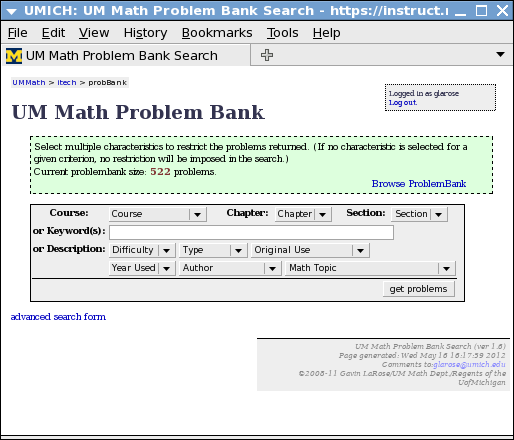
\includegraphics[height=2.5in]{um_search1}\quad
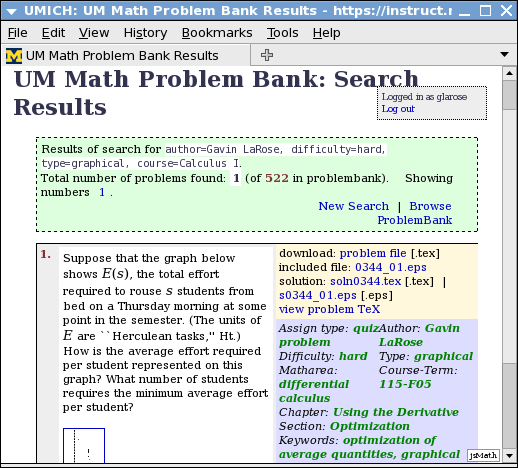
\includegraphics[height=2.5in]{um_result1}\\
\caption{UM Problem Library: left, search form; right, sample search result}
\label{umprobbank}
\end{center}
\end{figure}

The problem library in use in the mathematics department at the University
of Michigan is shown in Figure~\ref{umprobbank}, which shows the
search interface and a sample problem as displayed in a search result.
This illustrates in a general way the basic search characteristics that
will be supported by ROPE: the ability to locate problems that are
associated with specific topics in a course, which are of varying levels
of difficulty, that have specific characteristics (such as use of
graphically presented or tabular data), or which were used in specific
contexts (as homework problems, on quizzes, etc.).  This project will
dramatically rework this application, allowing it to address the goals
that are laid out in the introduction of this proposal, by including
\begin{itemize}
  \item
    scalability to support many more users, problems and problem formats,
  \item 
    community site membership and interactions,
  \item 
    problem moderation and editing,
  \item 
    problem filtering to generate alternate formats from existing
    formats,
  \item
    a modern, flexible interface that supports these features, and
  \item
    a well-documented API that will allow other applications to
    communicate with ROPE in manners other than through the browser
    interface.
\end{itemize}
These goals are described in greater detail in the following subsections.

\begin{subsection}{Scalability}

The problem library at the University of Michigan runs behind the
University web-login system and has access restricted to instructors in
the mathematics department. It accordingly supports a user base of several
hundred users, all of whom are defined by external data sources and need
no further identification or system characteristics. ROPE will support
thousands of users with internally defined characteristics (names, e-mail
addresses, password information, etc.). Accordingly, we will in the course
of the project expand the database used for the University of Michigan
system to support this. In addition, we will establish the workflow to
allow for users to author, submit and rate problems, determine the
appropriate manner in which moderation, editing of and commenting on
problems should take place, and add these functions to the problem code.

Problem types supported by the University of Michigan problem bank are
\LaTeX\ and external formats (\emph{Word} or \emph{OpenOffice} document
snippets). All problems for the problem bank are currently maintained as
separate files. For ROPE we will completely revise the problem data
structures so that all problem data are maintained in the system's
database, and completely rework the data maintained for problems to extend
the types of descriptive data for the problems and to support additional
file formats and the ability to add additional formats as they become
useful.

\end{subsection}

\begin{subsection}{Community and Site Moderation}

An aspect that is missing from the current problem bank is a mechanism for
users to provide feedback on the quality and usefulness of problems. ROPE will address this by including the ability for users to vote and
comment on problems in the library.  The data management and manner in
which this is to be done will be added to the current problembank
model.  In addition, problem view/download statistics will be provided as
part of the metadata about problems.

We will determine the nature of the voting/commenting system used, in
consultation with the Advisory Group, with the goal of maximizing its
usefulness and minimizing the possibility of any abuse. ROPE will also
support comment and problem flagging so that problems or comments with
errors can be updated by ROPE moderators. We anticipate that the moderators
will initially be drawn from the grant personnel, and will work with the
Advisory Group to determine the best manner to expand the group of people
who are engaged in this activity.  (We discuss the project's Advisory
Group in the following sections.)  ROPE will also support problem
authoring or submission from users in its community.  The degree of
moderation for this activity (if any) will also be determined by the
project personnel, including our Advisory Group.

In addition, ROPE will support a sharable problem collection feature.
This will allow users to create problem lists for their own
uses---homework sets for given courses, etc.---and to share these lists.
Thus an instructor teaching a course will be able to share her/his problem
lists with other faculty at her/his institution, or with colleagues at
other institutions.  In addition, book authors (and publishers) could
build problem lists for their texts that would then be openly available
for anyone using those texts.

\end{subsection}

\begin{subsection}{Problem Filtering}

As we add additional problem formats to ROPE, we will build in the
ability to convert between some of the formats and output types, and to
add additional filters as they are needed and developed. We anticipate
three initial filters:
\begin{itemize}
  \item
    a filter converting \TeX\ formatted problems to PDF output;
  \item
    a filter converting \TeX\ formatted problems to a rudimentary WeBWorK
    problem file; and
  \item
    a filter converting WeBWorK formatted problems to \TeX\ output. 
\end{itemize}
These will serve to provide significant additional functionality to ROPE and will be templates that illustrate the manner in which additional
filters may be constructed.

\end{subsection}

\begin{subsection}{Interface}

Considering these features and goals, it is clear that the simple search
and results interface used by the University of Michigan problem bank
system (Figure~\ref{umprobbank}) will need to be completely re-imagined.
We, with our Advisory Group, will work to develop an entirely new
interface that supports the precision of searching that we need and the
multitude of new data and features that ROPE will support.

\end{subsection}

\begin{subsection}{API and Documentation}

A natural extension to the filtering system that will be developed for ROPE is a mechanism by which other applications can use the generated
problem formats. To allow this, we will develop an easily used API by
which external applications may query ROPE to get file or problem data
for specified problems. A first application for this will be to allow the
open-source web homework system WeBWorK to include problems drawn from ROPE.  We will work with WeBWorK developers and the WeBWorK leadership
group on this aspect of the project.

\end{subsection}

\end{section}

\begin{section}{Intellectual Merit}

ROPE project will address a current need in undergraduate mathematics
education: the need for a widely available source of good problems that
instructors can use in a variety of educational venues.  Much of the
learning that takes place in mathematics, and other STEM fields, is driven
by students' work, and the success of that learning is fundamentally
dependent on the types of problems on which they work.  We therefore
expect ROPE to have the potential to be a significant and widely used
tool to enhance student learning.  

There are several specific aspects of ROPE which will have direct
bearing on this.
\begin{itemize}
  \item
    Its online search page that allows precise searches for specific
    types of problems.
  \item
    The open nature of the system that allows a wide range of uses of the
    problems in the library.
  \item
    The user feedback and statistics available for the problems in the
    library. 
  \item
    Users' ability to create their own problem sets, and to share
    these with other users.
  \item
    The explicitly extensible design of the system, allowing multiple
    problem formats and conversions between them.
\end{itemize}

Taking these together, we expect that ROPE will develop into an
easy-to-use, widely adopted resource with a correspondingly significant
impact on student learning of undergraduate mathematics.

\end{section}

\begin{section}{Broader Impacts}

The broad impact of ROPE will stem from its accessibility, ease-of-use
and extensibility.  We believe that the features that we are including in
ROPE will result in its use by many faculty at many institutions.  We
expect that the largest group of users of ROPE will be faculty who are
browsing for additional homework, test or quiz problems for their courses.
Even with a well-written textbook there are routine and inevitable cases
in an instructor will be at a loss to find a problem that s/he likes, and
ROPE will be the perfect resource to fill that gap.  In addition, as
open-content textbooks expand in popularity and availability, the
usefulness of ROPE will similarly increase.  We anticipate that
textbook authors may choose to define problem sets in ROPE for use by
instructors using their texts whether they are publishing open-content
textbooks or working with a publisher (though it is clear that the
attractiveness of ROPE to the former may be significantly greater).
And because ROPE will be designed from the outset to be flexible and
extensible, it will be able to meet the changing needs of faculty in the
future and make connections with other software projects for which a
library of open problems will be useful.

All told, we expect that ROPE should have very broad impact, reaching
instructors at all types of colleges and universities who are teaching any
standard mathematics course in any of a number of different ways.  We
further expect that as ROPE develops we will be able to extend it to
include other disciplines, also increasing its impact.

\end{section}

